\subsection{Maximum Speed}
\label{sec:speed}
When an object is outside the range of sensors it is said to be vacant.
When an object is in a vacant time interval its position can be narrowed down to the cell it is located in. 
further it can be narrowed down based on the max speed of the object denoted is $V_{max}*\Delta t_1$ . 
The speed of a object type may vary, e.g. a human have a max speed of 37.58 km/h~\cite{bolt}.
We view the range of the sensor $s$ as a circle with the sensors maximum range as radius, we call this $r_1$. 
Knowing the maximum speed of the object a circle can be drawn from the point where the object left the vicinity of the sensor.
This circle is the area where the object is located. 
It is, however, not know the point of exit from the sensor but only that the object left. 
The area of the object can then be calculated by creating a circle with the maximum sensor range plus the maximum range that the object can have traveled. 
The next reading of the object can be used to create a oval between the two sensor readings.  

\begin{figure}%
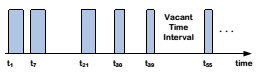
\includegraphics[width=\columnwidth]{images/vacant.png}%
\caption{}%
\label{fig:vacant}%
\end{figure}


\begin{figure}%
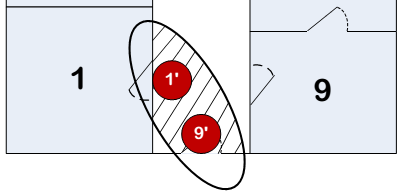
\includegraphics[width=0.8\columnwidth]{images/speed2.png}%
\caption{}%
\label{fig:speed2}%
\end{figure}




\begin{figure}%
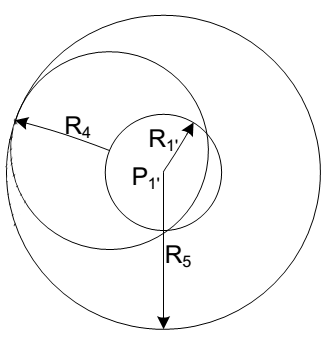
\includegraphics[width=\columnwidth]{images/speed.png}%
\caption{}%
\label{}%
\end{figure}
